\subsection{Threshold shift at finite size}\label{sec:threshold}
At finite $M$, the failure probability at $r=0$ is not equal to $1/2$. We use the 112 rows of
central-window data ($|z_0|\le2$, $k=3$--$6$, $M=64$--$262144$) to test this shift, converting
in three steps. First we approximate the probability of duplicate edges by
$p_{\rm dup}=1-e^{-\lambda}$, where $\lambda=\binom d2/\binom Mk$. Then, assuming the
macro-core event and the duplicate-edge event are approximately independent, we convert to the
macro failure probability $p_{\rm core}=(\widehat p_F-p_{\rm dup})/(1-p_{\rm dup})$. Finally we
set $z_{\rm emp}=\Phi^{-1}(p_{\rm core})$ (Figure~\ref{fig:threshold}).

For $M\ge1024$, the measured shift $z_{\rm emp}-z_0$ is 94\%--101\% of the analytic prediction
$C_kM^{-1/6}$; including all data, the ratio is 88\%--103\%. Using only $z_0$, even at
$M=262144$ the mean absolute error of the failure probability remains 0.06--0.10; after
switching to $z_{\rm sh}$, the error does not exceed 0.008 for $M\ge4096$. For example, at
$k=3$, $r=0$, $M=65536$, the measured failure rate is 0.617 while $\Phi(z_{\rm sh})=0.619$.
After the shift, the residual for $M\ge4096$ is at most 0.06 on the $z$ scale, and the largest
residual appears at the window edge, with a direction and magnitude consistent with the known
finite-size bias of the window width.

These data support the following practice: in the tested Plain configurations, the shift
constant of the configuration model approximates the threshold center at finite size. This
conclusion is a numerical verification; whether the shift order transfers to the Plain model
still requires a separate proof. Together with Appendix~\ref{sec:convergence}, this section
separates two finite-size effects: the shift of the threshold center is captured by the
translation, while the bias of the conditional distribution itself at a fixed failure
probability is unaffected by the translation and is examined separately.
\begin{figure}[!htbp]
\centering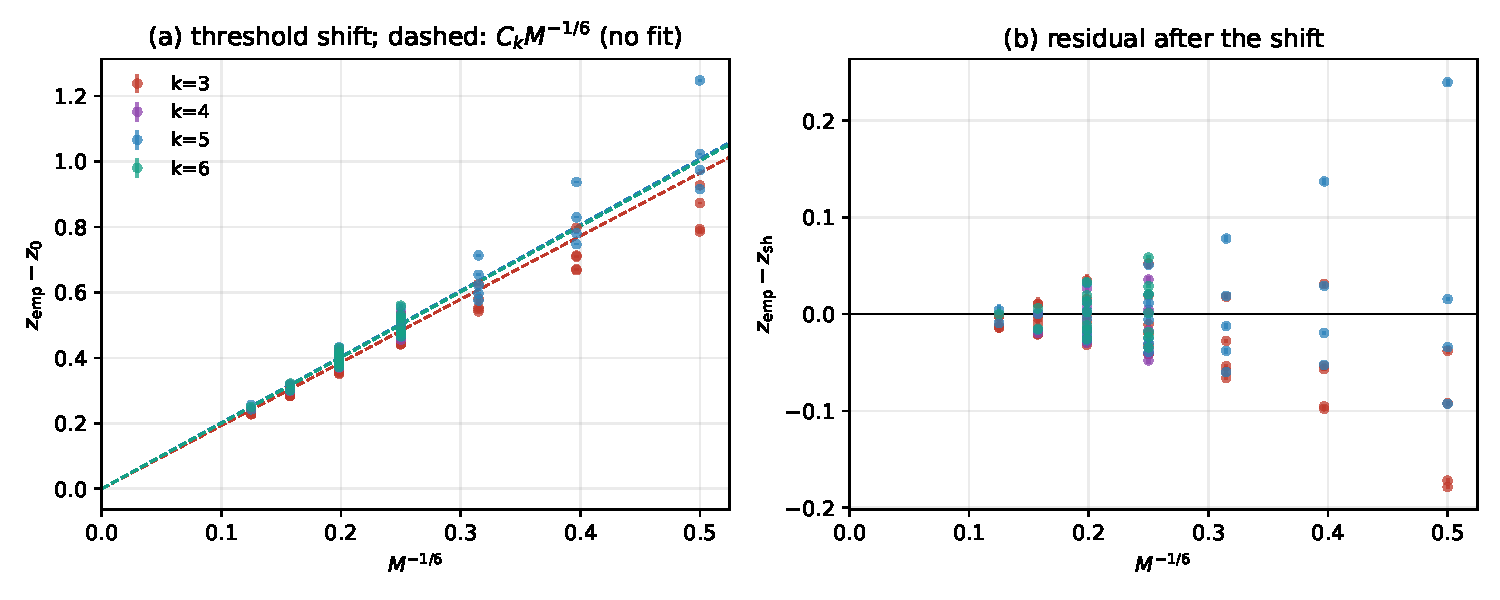
\includegraphics[width=\linewidth]{figures/fig_threshold.pdf}
\caption{Location of the threshold center. (a) measured shift and the analytic prediction
$C_kM^{-1/6}$ (dashed); (b) residual after the shift.}
\label{fig:threshold}
\end{figure}

\subsection{Chi-square shape of the unconditional measurement}\label{sec:chisq}
Under balanced signs, failure selection does not operate, so the shape of the unconditional
measurement at finite size can be tested separately. We compare its empirical quantile with the
quantile $[\chi^2_{M-1,u}-(M-1)]/\sqrt{2(M-1)}$ of the standardized chi-square $(M-1)$,
without fitting any parameters (Figure~\ref{fig:chisq}). For $k=3$ and $u=0.01$, at
$M=64,256,1024,4096,65536$ the measured quantiles are $-2.058$, $-2.205$, $-2.255$, $-2.293$,
$-2.319$; the chi-square gives $-2.064$, $-2.196$, $-2.261$, $-2.294$, $-2.318$; the normal
quantile is $-2.326$. The cases $k=4,5,6$ and $u=0.05$ likewise agree to about $0.01$.

Thus even at critical load, where the count of a single cell is far from normal, the shape at
finite $M$ is consistent with the chi-square inheritance obtained under deep overload in
\cite{prior}. The standardized chi-square has skewness $\sqrt{8/(M-1)}$, which vanishes as $M$
grows, consistent with the normal limit of Theorem~\ref{thm:main}. This yields the shape
correction $\kappa(u)$ of Section~\ref{sec:rules}, which contains no fitted parameters. The
chi-square result of \cite{prior} fixes $M$ and increases the load; here $M$ and $d$ grow
together. The agreement provides an empirical bridge between the two limiting orders.
\begin{figure}[!htbp]
\centering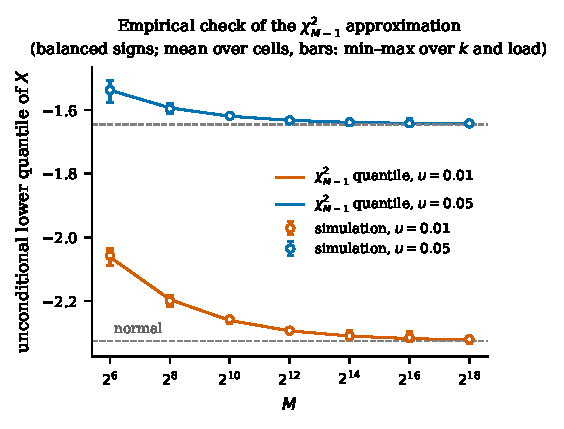
\includegraphics[width=.8\linewidth]{figures/fig_chisq.pdf}
\caption{Lower quantile of the unconditional measurement under balanced signs, and the
standardized chi-square $(M-1)$ quantile.}
\label{fig:chisq}
\end{figure}
